
\textbf{Oversikt}

Skissen under illustrerer hvordan informasjon relatert til ulike land kan framstilles med datasettene. Her er det tenkt at når man velger et land ut ifra listen, vil vinduene til høyre og under oppdateres med ulik informasjon som benytter data fra alle datasettene.

\textit{Student performance} vil gi en gruppert oversikt over studenters ytelse på skolen, og hvilke faktorer som påvirker karakterene deres. Utregningene gjennomføres ved å finne gjennomsnittskarakter etter mor og fars utdanningsnivå eller elevens fritidsnivå. Dette fremstilles da visuelt med grafer.

\textit{Country profiles} er hvert land sin overordnede socio-økonomiske profil. Her legger vi land i lister etter gdp per capita, hvor dyrt det er å bo i landet, og hvor landet tjener på skatt.

\textit{World university ranking} vil vise lister over skolerangering etter kjønnsfordeling og gjennomsnitt beregnet "score", basert på hvilket land man velger, eller om man browser skoler og utdanning.

Til slutt har vi \textit{Reigns og Regime} settene hvor vi ser på regimetype popularitet gjennom tidene hvor vi ser hvordan politikken utvikler seg på en internasjonal skala.

\textbf{Forside}

Her er en skisse som viser hvordan forsiden kan se ut. Det vil være et søkefelt der man kan søke etter land og skoler. Under søkefeltet vises det statistikk som bruker kan klikke seg inn på, blant annet for å komme til land-siden.

Vi kan for eksempel, vise anbefalte skoler basert på kjønnsfordeling eller hvilken land det lønner seg å søke jobb i.

\FigureCounter
\begin{figure}[H]
    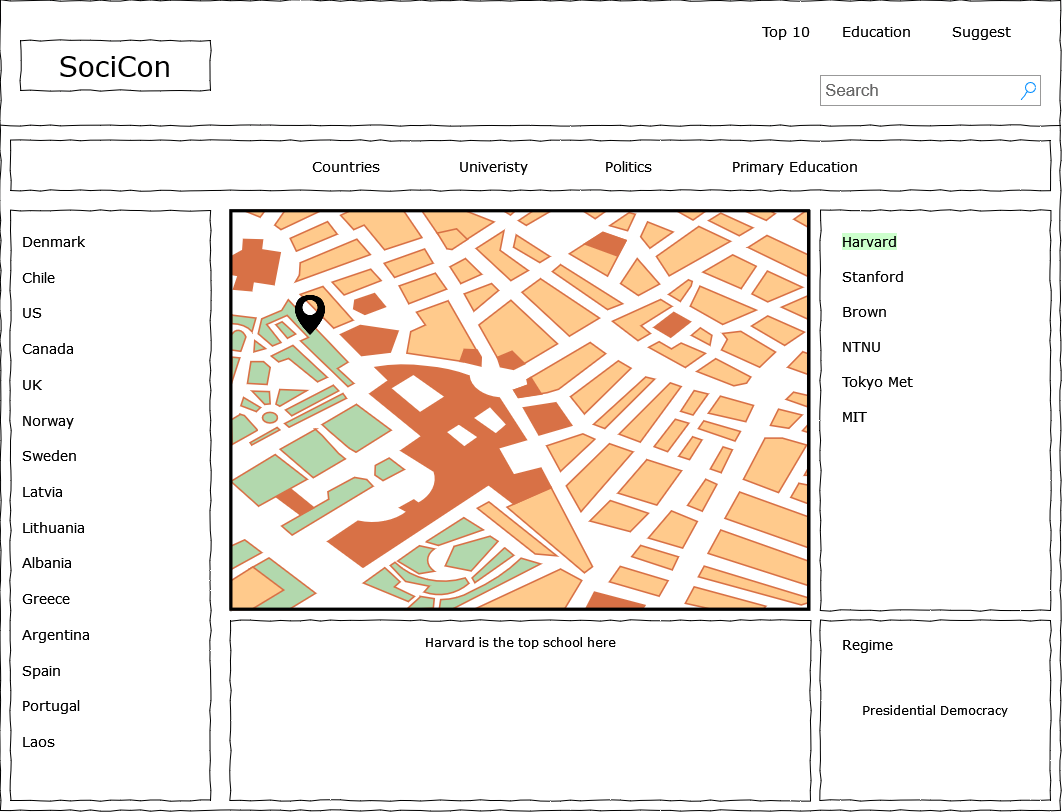
\includegraphics[width=\textwidth]{images/milepael1/forsideBigdata.png}
\end{figure}
